\vspace{-0.1cm}
\section{Application to Real Data}
\label{sec:application}

\begin{wrapfigure}{l}{0.45\textwidth}
  \vspace{-0.4cm}
  \centering
  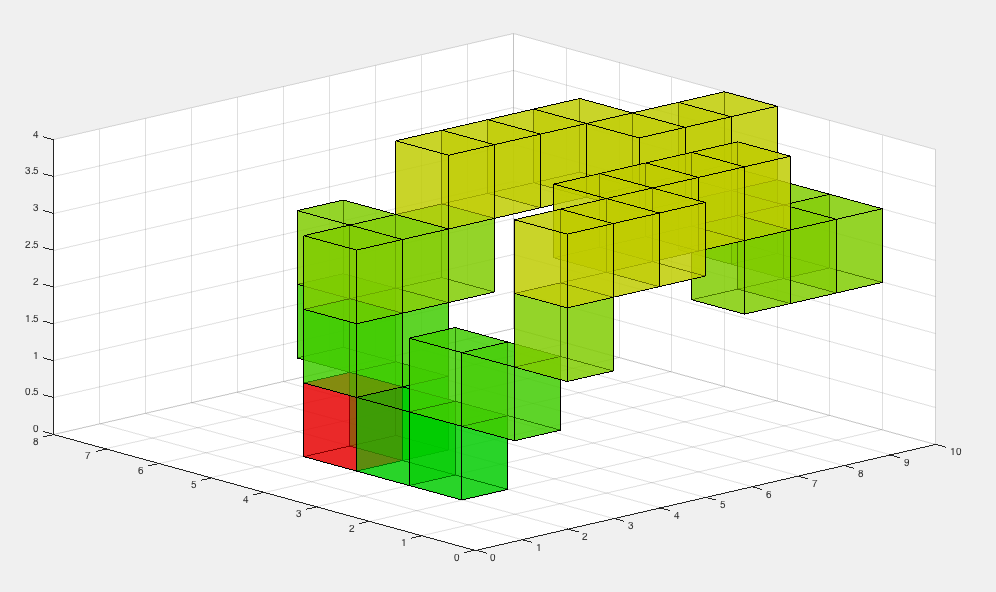
\includegraphics[width=0.45\textwidth]{./figures/returnsHome}
    \caption{Trace modeling property $\phi_{returnsHome}$}
    \label{fig:returnsHome}
\end{wrapfigure}
In this section, we apply our tool to cases of real data.
Both examples utilize spatial traces gathered from a small flying robot (a quadrotor unmanned aerial vehicle, or UAV), flown inside a VICON motion capture room.
The trace file is originally a ROS .bag file, and is processed as discussed in Sec.~\ref{sec:tool}. 
Although not depicted in these visualizations, these paths are directed in ascending time. 

The first example considers one actor $\bigstar_i$ and the property $\phi_{\{returnsHome\}}$.  
As shown in Fig.~\ref{fig:returnsHome}, this property is true for a trace $T$ when an actor revisits the cube from which $T$ begins.
The UAV begins on the ground, flies up and across the space, translates in y, and then returns back to where it started from.
The cube at which $\phi_{returnsHome}$ became true is highlighted in the figure.
The unit cube size used in this example is $0.5m$, about the size of the UAV.
We chose this size for the cube because at this size, if the `fuzziness' property is $1$ and there is no intersection, then they could not collide.

\begin{wrapfigure}{r}{0.45\textwidth}
  \vspace{-0.4cm}
  \centering
  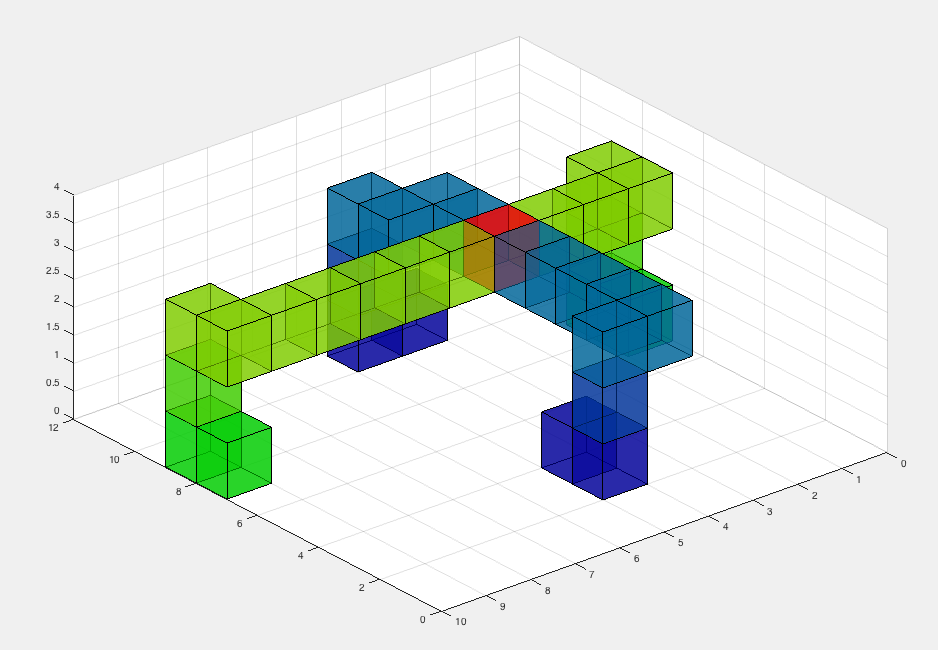
\includegraphics[width=0.45\textwidth]{./figures/independence.png}
  \caption{Trace modeling property $\phi_{\{independence\}} = false$}
    \label{fig:independence}
\end{wrapfigure}


The second example involves two UAVs, that together model the property $\phi_{\{independence\}}$.
This property is true of one or more traces $T$ when they crossed each other's space during any interval of the traces.
As shown in Fig.~\ref{fig:independence}, one UAV's path is shown moving from bottom left to upper right, and a second UAV's path moves from right to left.
The cube where $\phi_{\{independence\}}$ becomes false is highlighted in the figure.


Although these visualizations depict simple properties, they demonstrate that our tool correctly implements the technique and show the application to real data.
Note also that $\phi_{\{independence\}}$ is equivalent to $\phi_{\{k-independence\}}$ for $k=0$.
Both visualization are generated in MATLAB from a simple structured text file generated by \emph{Abstractus}.

